\chapter{La meiosis y la mezcla genética}\label{ch:g12:meiosis-genetic-shuffling}

Dos progenitores, cada uno con 46 \omterm{def:g10:universal-dna:information}{cromosomas}, producen un hijo con 46
--- y no con 92. En algún punto entre el cuerpo de los padres y el
hijo, el recuento se reduce a la mitad, y se reduce de una manera que
reparte a cada hijo una mano que ningún hermano ha tenido nunca: los
mismos padres, cuarenta años de hijos y ninguno igual a otro salvo los
gemelos idénticos. La reducción a la mitad es una división especial
llamada \omterm{def:g12:meiosis-genetic-shuffling:meiosis}{meiosis}; el reparto es lo que esa división hace con los
\omterm{def:g10:universal-dna:information}{cromosomas} por el camino. Este capítulo sigue a una \omterm{def:g10:cells-common-unit:cell}{célula} a lo largo
de la \omterm{def:g12:meiosis-genetic-shuffling:meiosis}{meiosis}, cuenta las combinaciones que puede producir y lee los
resultados de unos cruzamientos que revelan, desde fuera, lo que
ocurrió dentro.

\section{Reducir el juego a la mitad}

\begin{definition}[Diploide, haploide, meiosis]\label{def:g12:meiosis-genetic-shuffling:meiosis}
Una \omterm{def:g10:cells-common-unit:cell}{célula} que lleva dos copias de cada \omterm{def:g11:cell-cycle-mitosis:chromosome}{cromosoma} --- una de cada
progenitor, y las dos forman una pareja de \emph{\omterm{def:g10:universal-dna:information}{cromosomas} homólogos}
--- es \emph{diploide}\index{diploide}, y se escribe $2n$ ($2n = 46$ en
los humanos). Una \omterm{def:g10:cells-common-unit:cell}{célula} que lleva una copia de cada uno es
\emph{haploide}\index{haploide}, y se escribe $n$. La
\emph{meiosis}\index{meiosis} es la sucesión de dos divisiones por la
que una \omterm{def:g10:cells-common-unit:cell}{célula} diploide, tras una sola replicación de su \omterm{def:g10:universal-dna:information}{ADN}, produce
cuatro \omterm{def:g10:cells-common-unit:cell}{células} haploides --- los gametos, o sus precursores. La
\emph{fecundación} une dos gametos haploides y restablece el número
diploide: la alternancia de meiosis y fecundación es el ciclo de toda
\omterm{def:g10:biodiversity-scales:species}{especie} de reproducción sexual.
\end{definition}

\begin{proposition}[Las dos divisiones]\label{prop:g12:meiosis-genetic-shuffling:divisions}
Antes de la \omterm{def:g12:meiosis-genetic-shuffling:meiosis}{meiosis} se replica el \omterm{def:g10:universal-dna:information}{ADN}: cada \omterm{def:g11:cell-cycle-mitosis:chromosome}{cromosoma} tiene dos
\omterm{def:g11:cell-cycle-mitosis:chromosome}{cromátidas}. Después:
\begin{itemize}
  \item \emph{Primera división} (\omterm{def:g12:meiosis-genetic-shuffling:meiosis}{meiosis} I, \emph{reduccional}): los
        \omterm{def:g10:universal-dna:information}{cromosomas} homólogos se emparejan de dos en dos en el ecuador;
        los miembros de cada pareja son arrastrados a polos opuestos.
        Cada \omterm{def:g10:cells-common-unit:cell}{célula} hija recibe \emph{un \omterm{def:g11:cell-cycle-mitosis:chromosome}{cromosoma} de cada pareja},
        todavía formado por dos \omterm{def:g11:cell-cycle-mitosis:chromosome}{cromátidas}: $n$ \omterm{def:g10:universal-dna:information}{cromosomas}, cantidad de
        \omterm{def:g10:universal-dna:information}{ADN} $q$ (la de una \omterm{def:g10:cells-common-unit:cell}{célula} \omterm{def:g12:meiosis-genetic-shuffling:meiosis}{diploide} antes de la replicación).
  \item \emph{Segunda división} (\omterm{def:g12:meiosis-genetic-shuffling:meiosis}{meiosis} II, \emph{ecuacional}): como
        en una \omterm{def:g11:cell-cycle-mitosis:cycle}{mitosis}, se separan las \omterm{def:g11:cell-cycle-mitosis:chromosome}{cromátidas} de cada \omterm{def:g11:cell-cycle-mitosis:chromosome}{cromosoma}.
        Cada una de las cuatro \omterm{def:g10:cells-common-unit:cell}{células} recibe $n$ \omterm{def:g10:universal-dna:information}{cromosomas} de una
        sola \omterm{def:g11:cell-cycle-mitosis:chromosome}{cromátida}, con una cantidad de \omterm{def:g10:universal-dna:information}{ADN} $q/2$.
\end{itemize}
La primera división reduce a la mitad el número de \omterm{def:g10:universal-dna:information}{cromosomas}; la
segunda reduce a la mitad la cantidad de \omterm{def:g10:universal-dna:information}{ADN}, hasta una \omterm{def:g11:cell-cycle-mitosis:chromosome}{cromátida} por
\omterm{def:g11:cell-cycle-mitosis:chromosome}{cromosoma}.
\end{proposition}
\admitted

\begin{omfigure}
\begin{tikzpicture}[font=\small, line cap=round]
  \tikzset{cellb/.style={draw, thick, fill=omDef!5, rounded corners=9pt, minimum width=2.5cm, minimum height=2.5cm},
           ma/.style={line width=3pt, omDef!80}, mb/.style={line width=3pt, omThm!80},
           mA/.style={line width=3pt, omDef!35}, mB/.style={line width=3pt, omThm!35}, cen/.style={fill=black}}
  % panel 1: diploid cell after S: two pairs (long pair blue, short pair red); paternal dark, maternal pale
  \begin{scope}
    \node[cellb] at (0,0) {};
    \draw[ma] (-0.75,0.7) .. controls (-0.62,0.1) .. (-0.75,-0.5); \draw[ma] (-0.49,0.7) .. controls (-0.62,0.1) .. (-0.49,-0.5); \fill[cen] (-0.62,0.1) circle (1.6pt);
    \draw[mA] (-0.2,0.7) .. controls (-0.07,0.1) .. (-0.2,-0.5); \draw[mA] (0.06,0.7) .. controls (-0.07,0.1) .. (0.06,-0.5); \fill[cen] (-0.07,0.1) circle (1.6pt);
    \draw[mb] (0.4,0.45) .. controls (0.53,0.1) .. (0.4,-0.25); \draw[mb] (0.66,0.45) .. controls (0.53,0.1) .. (0.66,-0.25); \fill[cen] (0.53,0.1) circle (1.6pt);
    \draw[mB] (0.9,0.45) .. controls (1.03,0.1) .. (0.9,-0.25); \draw[mB] (1.16,0.45) .. controls (1.03,0.1) .. (1.16,-0.25); \fill[cen] (1.03,0.1) circle (1.6pt);
    \node[anchor=north, align=center, font=\scriptsize, text width=3.05cm] at (0,-1.35) {tras la replicación:\\ $2n = 4$, ADN $2q$};
  \end{scope}
  % panel 2: metaphase I: pairs on the equator
  \begin{scope}[xshift=3.2cm]
    \node[cellb] at (0,0) {};
    \draw[dashed, gray] (-1.1,0) -- (1.1,0);
    \draw[ma] (-0.7,0.55) .. controls (-0.57,0.1) .. (-0.7,-0.35); \draw[ma] (-0.44,0.55) .. controls (-0.57,0.1) .. (-0.44,-0.35); \fill[cen] (-0.57,0.15) circle (1.6pt);
    \draw[mA] (-0.7,-0.05) .. controls (-0.57,-0.5) .. (-0.7,-0.95); \draw[mA] (-0.44,-0.05) .. controls (-0.57,-0.5) .. (-0.44,-0.95); \fill[cen] (-0.57,-0.15) circle (1.6pt);
    \draw[mb] (0.45,0.5) .. controls (0.58,0.2) .. (0.45,-0.1); \draw[mb] (0.71,0.5) .. controls (0.58,0.2) .. (0.71,-0.1); \fill[cen] (0.58,0.15) circle (1.6pt);
    \draw[mB] (0.45,0.1) .. controls (0.58,-0.2) .. (0.45,-0.5); \draw[mB] (0.71,0.1) .. controls (0.58,-0.2) .. (0.71,-0.5); \fill[cen] (0.58,-0.15) circle (1.6pt);
    \node[anchor=north, align=center, font=\scriptsize, text width=3.05cm] at (0,-1.35) {meiosis I: parejas de\\ homólogos en el ecuador};
  \end{scope}
  % panel 3: two cells after MI, each n=2 with two chromatids
  \begin{scope}[xshift=6.4cm]
    \node[cellb, minimum height=1.15cm] at (0,0.7) {};
    \node[cellb, minimum height=1.15cm] at (0,-0.7) {};
    \draw[ma] (-0.55,1.15) .. controls (-0.42,0.7) .. (-0.55,0.25); \draw[ma] (-0.29,1.15) .. controls (-0.42,0.7) .. (-0.29,0.25); \fill[cen] (-0.42,0.7) circle (1.6pt);
    \draw[mB] (0.35,1.0) .. controls (0.48,0.7) .. (0.35,0.4); \draw[mB] (0.61,1.0) .. controls (0.48,0.7) .. (0.61,0.4); \fill[cen] (0.48,0.7) circle (1.6pt);
    \draw[mA] (-0.55,-0.25) .. controls (-0.42,-0.7) .. (-0.55,-1.15); \draw[mA] (-0.29,-0.25) .. controls (-0.42,-0.7) .. (-0.29,-1.15); \fill[cen] (-0.42,-0.7) circle (1.6pt);
    \draw[mb] (0.35,-0.4) .. controls (0.48,-0.7) .. (0.35,-1.0); \draw[mb] (0.61,-0.4) .. controls (0.48,-0.7) .. (0.61,-1.0); \fill[cen] (0.48,-0.7) circle (1.6pt);
    \node[anchor=north, align=center, font=\scriptsize, text width=3.05cm] at (0,-1.35) {dos células: $n = 2$,\\ dos cromátidas, ADN $q$};
  \end{scope}
  % panel 4: four cells after MII, single chromatids
  \begin{scope}[xshift=9.6cm]
    \foreach \y in {1.05,0.35,-0.35,-1.05} \node[cellb, minimum height=0.6cm, minimum width=2.3cm] at (0,\y) {};
    \draw[ma] (-0.5,1.3) -- (-0.5,0.8); \fill[cen] (-0.5,1.05) circle (1.4pt); \draw[mB] (0.4,1.22) -- (0.4,0.88); \fill[cen] (0.4,1.05) circle (1.4pt);
    \draw[ma] (-0.5,0.6) -- (-0.5,0.1); \fill[cen] (-0.5,0.35) circle (1.4pt); \draw[mB] (0.4,0.52) -- (0.4,0.18); \fill[cen] (0.4,0.35) circle (1.4pt);
    \draw[mA] (-0.5,-0.1) -- (-0.5,-0.6); \fill[cen] (-0.5,-0.35) circle (1.4pt); \draw[mb] (0.4,-0.18) -- (0.4,-0.52); \fill[cen] (0.4,-0.35) circle (1.4pt);
    \draw[mA] (-0.5,-0.8) -- (-0.5,-1.3); \fill[cen] (-0.5,-1.05) circle (1.4pt); \draw[mb] (0.4,-0.88) -- (0.4,-1.22); \fill[cen] (0.4,-1.05) circle (1.4pt);
    \node[anchor=north, align=center, font=\scriptsize, text width=3.05cm] at (0,-1.45) {cuatro gametos: $n = 2$,\\ una cromátida, ADN $q/2$};
  \end{scope}
\end{tikzpicture}

{\small La \omterm{def:g12:meiosis-genetic-shuffling:meiosis}{meiosis} en una \omterm{def:g10:cells-common-unit:cell}{célula} con dos parejas de \omterm{def:g10:universal-dna:information}{cromosomas}
($2n = 4$); los tonos oscuros y claros marcan los dos miembros de cada
pareja, procedentes de los dos progenitores. La primera división separa
los homólogos y la segunda las \omterm{def:g11:cell-cycle-mitosis:chromosome}{cromátidas}. Aquí el \omterm{def:g11:cell-cycle-mitosis:chromosome}{cromosoma} largo
oscuro fue con el corto claro: uno de los dos repartos posibles.}
\end{omfigure}

\begin{omfigure}
\begin{tikzpicture}
\begin{axis}[
  width=0.88\linewidth, height=5.2cm,
  axis x line=bottom, axis y line=left,
  xmin=0, xmax=10, ymin=0, ymax=2.7,
  xlabel={tiempo}, ylabel={ADN por célula},
  xlabel style={font=\small, at={(axis description cs:0.5,-0.1)}, anchor=north},
  ylabel style={font=\small},
  tick label style={font=\small}, xtick=\empty,
  ytick={0.5,1,2}, yticklabels={$q/2$, $q$, $2q$},
  clip=false,
]
\addplot[thick, omDef] coordinates {(0,1) (2,1) (4,2) (5.9,2) (6,1) (7.9,1) (8,0.5) (10,0.5)};
\draw[dashed, gray] (axis cs:2,0) -- (axis cs:2,2.2); \draw[dashed, gray] (axis cs:4,0) -- (axis cs:4,2.2);
\draw[dashed, gray] (axis cs:6,0) -- (axis cs:6,2.2); \draw[dashed, gray] (axis cs:8,0) -- (axis cs:8,2.2);
\node[font=\small, anchor=south] at (axis cs:1,2.25) {$2n$, $q$};
\node[font=\small, anchor=south] at (axis cs:3,2.25) {fase S};
\node[font=\small, anchor=south] at (axis cs:5,2.25) {$2n$, $2q$};
\node[font=\small, anchor=south, omThm] at (axis cs:6,2.45) {meiosis~I};
\node[font=\small, anchor=south] at (axis cs:7,2.25) {$n$, $q$};
\node[font=\small, anchor=south, omThm] at (axis cs:8,2.45) {meiosis~II};
\node[font=\small, anchor=south] at (axis cs:9,2.25) {$n$, $q/2$};
\end{axis}
\end{tikzpicture}

{\small El \omterm{def:g10:universal-dna:information}{ADN} por \omterm{def:g10:cells-common-unit:cell}{célula} a lo largo de la \omterm{def:g12:meiosis-genetic-shuffling:meiosis}{meiosis}. Una replicación y
después dos divisiones sin replicación entre ellas: los gametos tienen
una cuarta parte del \omterm{def:g10:universal-dna:information}{ADN} que tenía la \omterm{def:g10:cells-common-unit:cell}{célula} madre tras la fase S, y la
mitad del que tiene en reposo una \omterm{def:g10:cells-common-unit:cell}{célula} \omterm{def:g12:meiosis-genetic-shuffling:meiosis}{diploide}.}
\end{omfigure}

\begin{example}[Las cifras humanas]\label{ex:g12:meiosis-genetic-shuffling:numbers}
Una \omterm{def:g10:cells-common-unit:cell}{célula} germinal del testículo, $2n = 46$, se replica hasta tener 46
\omterm{def:g10:universal-dna:information}{cromosomas} de dos \omterm{def:g11:cell-cycle-mitosis:chromosome}{cromátidas} ($2q$); tras la \omterm{def:g12:meiosis-genetic-shuffling:meiosis}{meiosis} I, dos \omterm{def:g10:cells-common-unit:cell}{células} de
23 \omterm{def:g10:universal-dna:information}{cromosomas} de dos \omterm{def:g11:cell-cycle-mitosis:chromosome}{cromátidas} ($q$); tras la \omterm{def:g12:meiosis-genetic-shuffling:meiosis}{meiosis} II, cuatro
espermatozoides de 23 \omterm{def:g10:universal-dna:information}{cromosomas} de una sola \omterm{def:g11:cell-cycle-mitosis:chromosome}{cromátida} ($q/2$). En la
fecundación, $23 + 23 =
46$ y $q/2 + q/2 = q$: el cigoto vuelve a ser
una \omterm{def:g10:cells-common-unit:cell}{célula} \omterm{def:g12:meiosis-genetic-shuffling:meiosis}{diploide} en reposo. En el ovario, esas mismas divisiones
producen un ovocito grande y tres \omterm{def:g10:cells-common-unit:cell}{células} diminutas que se descartan;
la aritmética es idéntica.
\end{example}

\section{La mezcla}

\begin{proposition}[Segregación independiente]\label{prop:g12:meiosis-genetic-shuffling:assortment}
En la metafase I, cada pareja de homólogos se alinea en el ecuador con
independencia de las demás parejas: qué miembro de una pareja va a qué
polo lo decide el azar, pareja por pareja. Una \omterm{def:g10:cells-common-unit:cell}{célula} con $n$ parejas
puede producir, por tanto, $2^n$ combinaciones distintas de \omterm{def:g10:universal-dna:information}{cromosomas}
paternos y maternos en sus gametos --- $2^{23} \approx \num{8.4e6}$ en
un humano. La fecundación, que une dos gametos así al azar, da $2^{23}
\times 2^{23} \approx \num{7e13}$ combinaciones de \omterm{def:g10:universal-dna:information}{cromosomas} para los
hijos de una pareja, antes de contar cualquier otra fuente de
variedad.
\end{proposition}
\admitted

\begin{proposition}[El entrecruzamiento]\label{prop:g12:meiosis-genetic-shuffling:crossingover}
Mientras los homólogos están emparejados, al principio de la \omterm{def:g12:meiosis-genetic-shuffling:meiosis}{meiosis} I,
dos \omterm{def:g11:cell-cycle-mitosis:chromosome}{cromátidas} no hermanas se rompen en el mismo punto y se vuelven a
unir cruzadas: es un
\emph{entrecruzamiento}\index{entrecruzamiento}. Cada \omterm{def:g11:cell-cycle-mitosis:chromosome}{cromátida}, más
allá del punto de intercambio, lleva ya los \omterm{def:g10:universal-dna:gene}{alelos} del otro homólogo.
Los \omterm{def:g10:universal-dna:information}{cromosomas} que llegan a los gametos no son, por tanto, los
\omterm{def:g10:universal-dna:information}{cromosomas} de los progenitores, sino \omterm{def:g10:universal-dna:information}{cromosomas}
\emph{recombinados}, que mezclan a lo largo de su longitud los \omterm{def:g10:universal-dna:gene}{alelos}
recibidos de los dos abuelos. En cada pareja y en cada \omterm{def:g12:meiosis-genetic-shuffling:meiosis}{meiosis} ocurren
de uno a tres intercambios, en posiciones variables: el número de
gametos posibles es, en la práctica, ilimitado.
\end{proposition}
\begin{proof}[Pruebas experimentales]
Al microscopio, los homólogos emparejados de la \omterm{def:g12:meiosis-genetic-shuffling:meiosis}{meiosis} I muestran
puntos cruzados, los \emph{quiasmas}, donde dos \omterm{def:g11:cell-cycle-mitosis:chromosome}{cromátidas} cambian de
pareja de forma visible. Los cruzamientos en los que dos \omterm{def:g10:universal-dna:gene}{genes} están en
el mismo \omterm{def:g11:cell-cycle-mitosis:chromosome}{cromosoma} dan, entre la descendencia, una minoría que lleva
combinaciones nuevas de los \omterm{def:g10:universal-dna:gene}{alelos} de esos dos \omterm{def:g10:universal-dna:gene}{genes} --- combinaciones
que no llevaba ninguno de los progenitores --- en una proporción que
depende de la distancia entre los \omterm{def:g10:universal-dna:gene}{genes}; los \omterm{def:g10:universal-dna:gene}{genes} muy separados en un
\omterm{def:g11:cell-cycle-mitosis:chromosome}{cromosoma} se recombinan tan a menudo como los \omterm{def:g10:universal-dna:gene}{genes} de \omterm{def:g10:universal-dna:information}{cromosomas}
distintos. Los marcadores moleculares seguidos en familias muestran que
los segmentos de cada \omterm{def:g11:cell-cycle-mitosis:chromosome}{cromosoma} cambian de origen abuelo en uno o dos
puntos por \omterm{def:g11:cell-cycle-mitosis:chromosome}{cromosoma} y generación.
\end{proof}

\begin{omfigure}
\begin{tikzpicture}[font=\small, line cap=round, >=Stealth]
  \tikzset{p/.style={line width=4pt, omDef!80}, m/.style={line width=4pt, omThm!70}}
  % before: two homologues, each two chromatids; alleles A/a, B/b
  \draw[p] (0,0) -- (0,3); \draw[p] (0.35,0) -- (0.35,3);
  \draw[m] (0.9,0) -- (0.9,3); \draw[m] (1.25,0) -- (1.25,3);
  \foreach \x in {0,0.35} { \node[font=\scriptsize, anchor=east, xshift=-1pt] at (\x,2.6) {}; }
  \node[font=\scriptsize, omDef!80!black, anchor=east] at (-0.15,2.6) {$A$};
  \node[font=\scriptsize, omDef!80!black, anchor=east] at (-0.15,0.5) {$B$};
  \node[font=\scriptsize, omThm!80!black, anchor=west] at (1.4,2.6) {$a$};
  \node[font=\scriptsize, omThm!80!black, anchor=west] at (1.4,0.5) {$b$};
  \node[anchor=north, align=center] at (0.62,-0.2) {homólogos emparejados\\ (dos cromátidas cada uno)};
  \draw[->, thick] (2.4,1.5) -- (3.4,1.5);
  % during: chiasma between the two inner chromatids at y=1.5
  \begin{scope}[xshift=4.2cm]
    \draw[p] (0,0) -- (0,3);
    \draw[p] (0.35,3) -- (0.35,1.6) -- (0.9,1.4) -- (0.9,0);
    \draw[m] (0.9,3) -- (0.9,1.6) -- (0.35,1.4) -- (0.35,0);
    \draw[m] (1.25,0) -- (1.25,3);
    \node[anchor=north, align=center] at (0.62,-0.2) {quiasma: dos cromátidas\\ se rompen y se unen cruzadas};
  \end{scope}
  \draw[->, thick] (6.6,1.5) -- (7.6,1.5);
  % after: four chromatids separated
  \begin{scope}[xshift=8.4cm]
    \draw[p] (0,0) -- (0,3);
    \draw[p] (0.5,3) -- (0.5,1.5); \draw[m] (0.5,1.5) -- (0.5,0);
    \draw[m] (1.0,3) -- (1.0,1.5); \draw[p] (1.0,1.5) -- (1.0,0);
    \draw[m] (1.5,0) -- (1.5,3);
    \node[font=\scriptsize, anchor=south] at (0,3.05) {$AB$};
    \node[font=\scriptsize, anchor=south] at (0.5,3.05) {$Ab$};
    \node[font=\scriptsize, anchor=south] at (1.0,3.05) {$aB$};
    \node[font=\scriptsize, anchor=south] at (1.5,3.05) {$ab$};
    \node[anchor=north, align=center] at (0.75,-0.2) {cuatro gametos: dos parentales,\\ dos recombinados};
  \end{scope}
\end{tikzpicture}

{\small \omterm{prop:g12:meiosis-genetic-shuffling:crossingover}{Entrecruzamiento} entre dos \omterm{def:g10:universal-dna:gene}{genes} $A$ y $B$ del mismo \omterm{def:g11:cell-cycle-mitosis:chromosome}{cromosoma}.
Dos de las cuatro \omterm{def:g11:cell-cycle-mitosis:chromosome}{cromátidas} intercambian sus extremos; de los cuatro
gametos, dos llevan las combinaciones parentales ($AB$, $ab$) y dos
otras nuevas ($Ab$, $aB$).}
\end{omfigure}

\begin{omfigure}
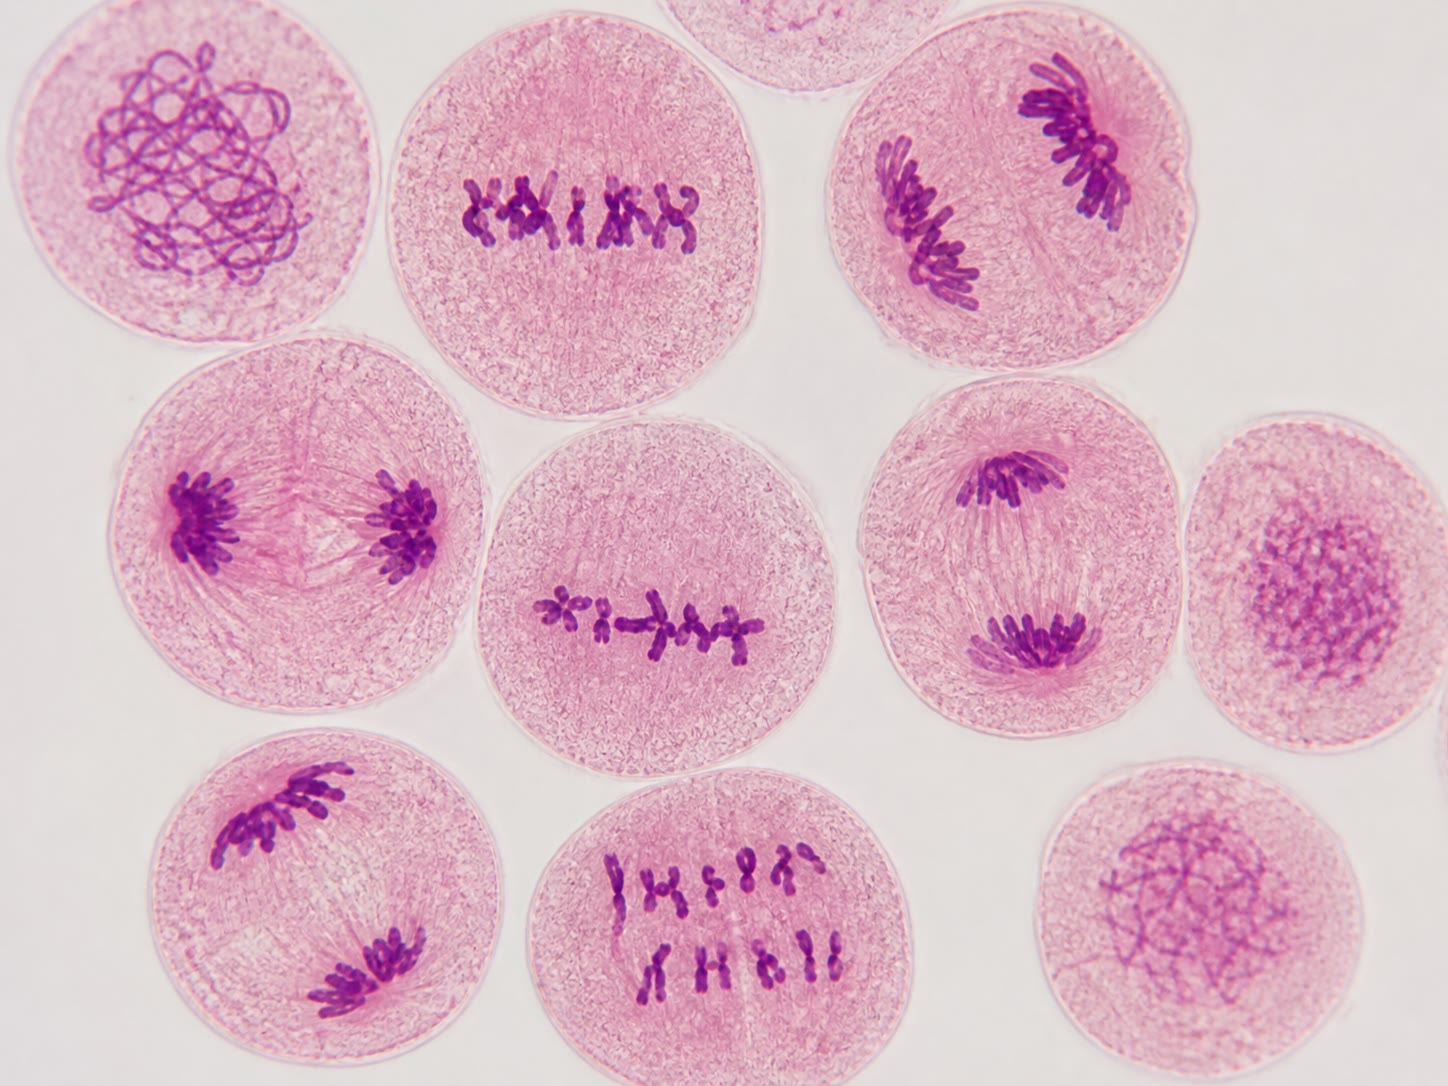
\includegraphics[width=0.56\linewidth]{images/book2/ai/g12-meiosis-lily-anther.jpg}

{\small \omterm{def:g10:cells-common-unit:cell}{Células} de una antera de lirio en \omterm{def:g12:meiosis-genetic-shuffling:meiosis}{meiosis}, teñidas: en unas,
los homólogos emparejados se alinean en mitad de la \omterm{def:g10:cells-common-unit:cell}{célula}; en otras
han sido arrastrados a los dos polos. Las etapas del esquema, vistas en
el tejido que fabrica el polen.}
\end{omfigure}

\begin{example}[Tres fuentes de variedad, en orden]\label{ex:g12:meiosis-genetic-shuffling:sources}
Un hijo de dos progenitores es nuevo de tres maneras: el
\omterm{prop:g12:meiosis-genetic-shuffling:crossingover}{entrecruzamiento} reconstruyó cada \omterm{def:g11:cell-cycle-mitosis:chromosome}{cromosoma} de cada gameto a partir de
las dos copias de los abuelos; la segregación independiente repartió en
el gameto un \omterm{def:g11:cell-cycle-mitosis:chromosome}{cromosoma} recombinado de cada pareja, entre $2^{23}$
repartos; y la fecundación unió uno de esos gametos con otro sacado de
los $2^{23}$ del otro progenitor. La \omterm{def:g11:mutations:mutation}{mutación}, que creó los \omterm{def:g10:universal-dna:gene}{alelos} que
se barajan, actúa en una escala de tiempo mucho más lenta: la mezcla es
lo que hace nueva cada generación con la misma baraja.
\end{example}

\section{Leer la mezcla en un cruzamiento}

\begin{omfigure}
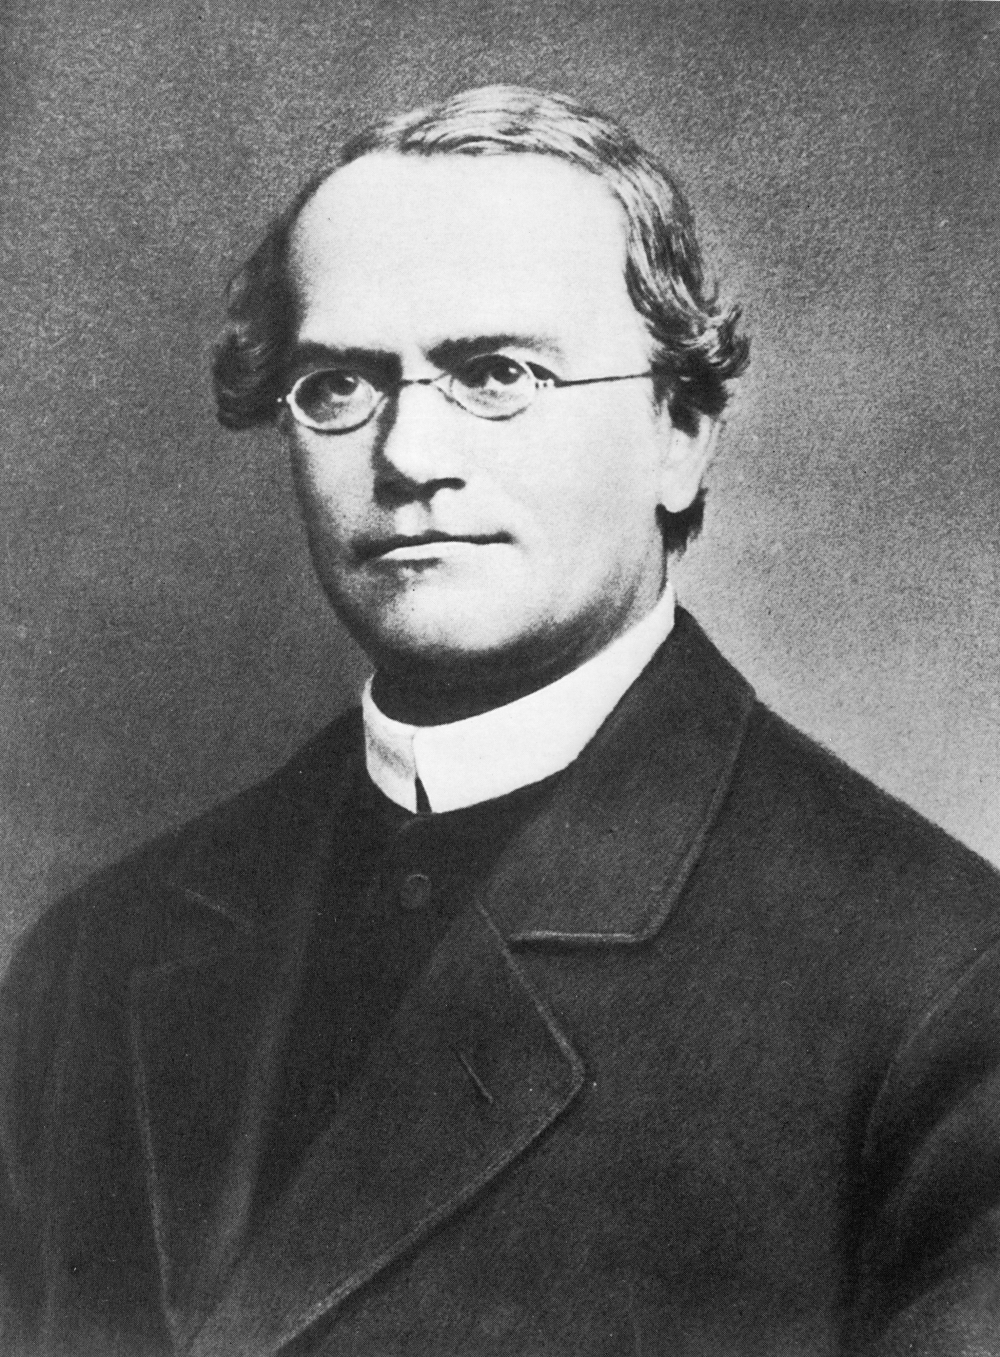
\includegraphics[width=0.3\linewidth]{images/book2/mendel.jpg}

{\small Gregor Mendel, que contó la descendencia de sus cruzamientos de guisantes en el jardín de un monasterio en los años sesenta del siglo XIX y encontró las proporciones --- 3:1 para un carácter, 9:3:3:1 para dos --- que produce la \omterm{def:g12:meiosis-genetic-shuffling:meiosis}{meiosis}, desconocida para él. Fotografía, dominio público.}
\end{omfigure}

\begin{method}[El cruzamiento de prueba]\label{met:g12:meiosis-genetic-shuffling:testcross}
Para ver qué gametos fabrica un individuo, se lo cruza con una pareja
que solo lleve \omterm{def:g10:universal-dna:gene}{alelos} \omterm{def:g11:genes-and-disease:genetic}{recesivos} (un \emph{cruzamiento de prueba}): cada
descendiente muestra entonces exactamente los \omterm{def:g10:universal-dna:gene}{alelos} que llevaba el
gameto del progenitor puesto a prueba. Para dos \omterm{def:g10:universal-dna:gene}{genes}, con el
progenitor probado $AaBb$ y la pareja $aabb$:
\begin{enumerate}
  \item Cuenta las cuatro clases de descendientes: $AB$, $Ab$, $aB$,
        $ab$ (cada uno lleva además $ab$ de la pareja).
  \item Si las cuatro son igual de frecuentes ($1:1:1:1$), los \omterm{def:g10:universal-dna:gene}{genes}
        están en \omterm{def:g10:universal-dna:information}{cromosomas} distintos y se segregan de forma
        independiente.
  \item Si dos clases (las combinaciones parentales) son mucho más
        frecuentes que las otras dos (las recombinantes), los \omterm{def:g10:universal-dna:gene}{genes}
        están en el mismo \omterm{def:g11:cell-cycle-mitosis:chromosome}{cromosoma}; las recombinantes vienen del
        \omterm{prop:g12:meiosis-genetic-shuffling:crossingover}{entrecruzamiento}, y su proporción mide la distancia entre los
        \omterm{def:g10:universal-dna:gene}{genes}.
  \item Las recombinantes son siempre la minoría y siempre vienen en
        dos clases iguales; las parentales, también.
\end{enumerate}
\end{method}

\begin{example}[Dos cruzamientos en la mosca de la fruta]\label{ex:g12:meiosis-genetic-shuffling:fly}
Mosca A, heterocigótica para el color del cuerpo y la forma del ala,
sometida a un cruzamiento de prueba: 254 gris-normal, 248
negro-vestigial, 251 gris-vestigial, 247 negro-normal --- cuatro clases
iguales, los \omterm{def:g10:universal-dna:gene}{genes} están en \omterm{def:g10:universal-dna:information}{cromosomas} distintos. Mosca B,
heterocigótica para el color del cuerpo y el color de los \omterm{def:g11:the-eye:parts}{ojos}: 412
gris-rojo, 405 negro-púrpura, 44 gris-púrpura, 39 negro-rojo --- dos
clases parentales de un 45\% cada una y dos clases recombinantes de un
5\%: los \omterm{def:g10:universal-dna:gene}{genes} están en el mismo \omterm{def:g11:cell-cycle-mitosis:chromosome}{cromosoma}, cerca uno de otro, y los
separa un \omterm{prop:g12:meiosis-genetic-shuffling:crossingover}{entrecruzamiento} en el 9\% de las \omterm{def:g12:meiosis-genetic-shuffling:meiosis}{meiosis}.
\end{example}

\begin{omfigure}
\begin{tikzpicture}[font=\small]
  \draw[thick] (0,0) grid[step=1.4] (5.6,1.4);
  \node[fill=omDef!15, minimum width=1.3cm, minimum height=1.3cm, align=center] at (0.7,0.7) {$AB$\\ 254};
  \node[fill=omDef!15, minimum width=1.3cm, minimum height=1.3cm, align=center] at (2.1,0.7) {$Ab$\\ 251};
  \node[fill=omDef!15, minimum width=1.3cm, minimum height=1.3cm, align=center] at (3.5,0.7) {$aB$\\ 247};
  \node[fill=omDef!15, minimum width=1.3cm, minimum height=1.3cm, align=center] at (4.9,0.7) {$ab$\\ 248};
  \node[anchor=south] at (2.8,1.5) {mosca A: genes independientes, $1:1:1:1$};
  \begin{scope}[xshift=7.4cm]
    \draw[thick] (0,0) grid[step=1.4] (5.6,1.4);
    \node[fill=omProp!25, minimum width=1.3cm, minimum height=1.3cm, align=center] at (0.7,0.7) {$AB$\\ 412};
    \node[fill=omThm!20, minimum width=1.3cm, minimum height=1.3cm, align=center] at (2.1,0.7) {$Ab$\\ 44};
    \node[fill=omThm!20, minimum width=1.3cm, minimum height=1.3cm, align=center] at (3.5,0.7) {$aB$\\ 39};
    \node[fill=omProp!25, minimum width=1.3cm, minimum height=1.3cm, align=center] at (4.9,0.7) {$ab$\\ 405};
    \node[anchor=south] at (2.8,1.5) {mosca B: genes ligados, parentales $\gg$ recombinantes};
  \end{scope}
\end{tikzpicture}

{\small Los gametos de dos moscas heterocigóticas, leídos en
cruzamientos de prueba. Clases iguales significan segregación
independiente; dos clases grandes y dos pequeñas significan que los
\omterm{def:g10:universal-dna:gene}{genes} están ligados, y las clases pequeñas las produce el
\omterm{prop:g12:meiosis-genetic-shuffling:crossingover}{entrecruzamiento}.}
\end{omfigure}

\section{Cuando la mezcla sale mal}

\begin{proposition}[Errores de la meiosis]\label{prop:g12:meiosis-genetic-shuffling:errors}
De vez en cuando, una pareja de homólogos no se separa en la \omterm{def:g12:meiosis-genetic-shuffling:meiosis}{meiosis} I,
o no lo hacen dos \omterm{def:g11:cell-cycle-mitosis:chromosome}{cromátidas} en la \omterm{def:g12:meiosis-genetic-shuffling:meiosis}{meiosis} II: un gameto recibe dos
copias de un \omterm{def:g11:cell-cycle-mitosis:chromosome}{cromosoma} y otro ninguna. Fecundados, dan un cigoto con
tres copias (\emph{trisomía}) o con una (\emph{monosomía}). Casi todos
esos cigotos no se desarrollan; los que lo hacen llevan un conjunto de
rasgos característicos. La trisomía 21 (alrededor de un nacimiento de
cada 700) causa discapacidad intelectual y defectos cardíacos y es la
más frecuente; su frecuencia sube abruptamente con la edad de la madre.
Un \omterm{prop:g12:meiosis-genetic-shuffling:crossingover}{entrecruzamiento} desigual --- \omterm{def:g11:cell-cycle-mitosis:chromosome}{cromátidas} que intercambian segmentos
desiguales --- produce un \omterm{def:g11:cell-cycle-mitosis:chromosome}{cromosoma} con un \omterm{def:g10:universal-dna:gene}{gen} duplicado y otro con una
deleción: el mecanismo por el que se multiplicaron los \omterm{def:g10:universal-dna:gene}{genes} de las
\omterm{def:g11:the-eye:photoreceptors}{opsinas} del \cref{ch:g11:the-eye}, y por el que aparecen \omterm{def:g10:universal-dna:gene}{genes} nuevos
(\cref{ch:g12:diversification-of-life}).
\end{proposition}
\admitted

\begin{omfigure}
\begin{tikzpicture}
\begin{axis}[
  width=0.84\linewidth, height=5.4cm,
  axis x line=bottom, axis y line=left,
  xmin=18, xmax=47, ymin=0, ymax=40,
  xlabel={edad de la madre (años)}, ylabel={trisomías 21 por 1000 nacimientos},
  xlabel style={font=\small, at={(axis description cs:0.5,-0.12)}, anchor=north},
  ylabel style={font=\small},
  tick label style={font=\small}, xtick={20,25,30,35,40,45}, ytick={0,10,20,30,40},
]
\addplot[thick, omThm, mark=*, mark size=1.5pt] coordinates
  {(20,0.7) (25,0.8) (30,1.1) (33,1.8) (35,2.9) (37,4.5) (39,7.5) (41,12) (43,20) (45,33)};
\end{axis}
\end{tikzpicture}

{\small Frecuencia de la trisomía 21 al nacer frente a la edad de la
madre. Los ovocitos se forman antes del nacimiento de la mujer y quedan
detenidos en la \omterm{def:g12:meiosis-genetic-shuffling:meiosis}{meiosis} I durante décadas; cuanto más larga es la
pausa, más probable es un fallo en la separación de los homólogos.}
\end{omfigure}

\begin{example}[Cromosomas sexuales mal contados]\label{ex:g12:meiosis-genetic-shuffling:sexchrom}
Un gameto sin \omterm{def:g11:cell-cycle-mitosis:chromosome}{cromosoma} sexual fecundado por otro \omterm{def:g11:genes-and-disease:genetic}{portador} de X da un
cigoto XO: una niña de estatura baja cuyos ovarios no se desarrollan.
Un óvulo XX fecundado por un espermatozoide Y da XXY: un niño cuyos
testículos siguen siendo pequeños y no fabrican espermatozoides. En los
dos casos, el \omterm{prop:g11:becoming-male-female:sry}{SRY} decide la gónada como en el
\cref{ch:g11:becoming-male-female}; el número de \omterm{def:g10:universal-dna:information}{cromosomas} X decide
buena parte del resto, y por eso estos son los más leves de los errores
cromosómicos.
\end{example}

\begin{remark}[Por qué el sexo]\label{rem:g12:meiosis-genetic-shuffling:whysex}
Una bacteria se copia a sí misma; un rosal puede crecer de un esqueje.
La reproducción sexual es más cara --- dos progenitores, una \omterm{def:g12:meiosis-genetic-shuffling:meiosis}{meiosis},
la búsqueda de pareja --- y su producto es una descendencia en la que
cada individuo es distinto de sus padres y de sus hermanos. Esa
diferencia es lo que importa: en un ambiente que cambia, y frente a
parásitos que evolucionan, una población de individuos variados tiene
más probabilidades de contener a algunos que sobrevivan que una
población de copias. La mezcla de este capítulo es la materia prima que
clasificará la selección de los dos capítulos siguientes.
\end{remark}

\section{Ejercicios}

\begin{exercise}[$\star$]\label{exo:g12:meiosis-genetic-shuffling:1}
Define \omterm{def:g12:meiosis-genetic-shuffling:meiosis}{diploide} y \omterm{def:g12:meiosis-genetic-shuffling:meiosis}{haploide}, y enuncia qué le hace la \omterm{def:g12:meiosis-genetic-shuffling:meiosis}{meiosis} al número
de \omterm{def:g10:universal-dna:information}{cromosomas} y a la cantidad de \omterm{def:g10:universal-dna:information}{ADN}.
\end{exercise}

\begin{exercise}[$\star$]\label{exo:g12:meiosis-genetic-shuffling:2}
¿Qué se separa en la \omterm{def:g12:meiosis-genetic-shuffling:meiosis}{meiosis} I? ¿Y en la \omterm{def:g12:meiosis-genetic-shuffling:meiosis}{meiosis} II? ¿Cuál es la
división reduccional?
\end{exercise}

\begin{exercise}[$\star$]\label{exo:g12:meiosis-genetic-shuffling:3}
Una \omterm{def:g10:cells-common-unit:cell}{célula} tiene $2n = 8$ y un \omterm{def:g10:universal-dna:information}{ADN} de $2q$ al empezar la \omterm{def:g12:meiosis-genetic-shuffling:meiosis}{meiosis}. Da el
número de \omterm{def:g10:universal-dna:information}{cromosomas} y la cantidad de \omterm{def:g10:universal-dna:information}{ADN} de las \omterm{def:g10:cells-common-unit:cell}{células} después de la
\omterm{def:g12:meiosis-genetic-shuffling:meiosis}{meiosis} I y después de la \omterm{def:g12:meiosis-genetic-shuffling:meiosis}{meiosis} II.
\end{exercise}

\begin{exercise}[$\star$]\label{exo:g12:meiosis-genetic-shuffling:4}
¿Cuántas combinaciones cromosómicas pueden mostrar los gametos de una
\omterm{def:g10:biodiversity-scales:species}{especie} con $2n = 8$ solo por segregación independiente?
\end{exercise}

\begin{exercise}[$\star$]\label{exo:g12:meiosis-genetic-shuffling:5}
¿Qué es un cruzamiento de prueba y qué revela la proporción de
descendientes recombinantes?
\end{exercise}

\begin{exercise}[$\star\star$]\label{exo:g12:meiosis-genetic-shuffling:6}
En la figura del \omterm{def:g10:universal-dna:information}{ADN}, lee el \omterm{def:g10:universal-dna:information}{ADN} por \omterm{def:g10:cells-common-unit:cell}{célula} de una \omterm{def:g10:cells-common-unit:cell}{célula} en \omterm{def:g12:meiosis-genetic-shuffling:meiosis}{meiosis} I,
de una \omterm{def:g10:cells-common-unit:cell}{célula} entre las dos divisiones y de un gameto. Explica por qué
no hay fase S entre las divisiones.
\end{exercise}

\begin{exercise}[$\star\star$]\label{exo:g12:meiosis-genetic-shuffling:7}
Un cruzamiento de prueba da 300 $AB$, 298 $ab$, 302 $Ab$, 300 $aB$.
¿Están ligados los \omterm{def:g10:universal-dna:gene}{genes}? ¿Cuáles son los gametos del progenitor?
\end{exercise}

\begin{exercise}[$\star\star$]\label{exo:g12:meiosis-genetic-shuffling:8}
Un cruzamiento de prueba da 460 $AB$, 455 $ab$, 42 $Ab$, 43 $aB$.
¿Están ligados los \omterm{def:g10:universal-dna:gene}{genes}? ¿Qué clases son recombinantes y qué fracción
suponen?
\end{exercise}

\begin{exercise}[$\star\star$]\label{exo:g12:meiosis-genetic-shuffling:9}
En la figura del \omterm{prop:g12:meiosis-genetic-shuffling:crossingover}{entrecruzamiento}, ¿qué dos gametos obtendrías si el
intercambio ocurriera \emph{por encima} de los dos \omterm{def:g10:universal-dna:gene}{genes}? Explícalo.
\end{exercise}

\begin{exercise}[$\star\star$]\label{exo:g12:meiosis-genetic-shuffling:10}
En la figura de la trisomía, lee la frecuencia a los 25, a los 35 y a
los 42 años, y calcula el factor entre los 25 y los 42.
\end{exercise}

\begin{exercise}[$\star\star$]\label{exo:g12:meiosis-genetic-shuffling:11}
Explica en qué se diferencia una no disyunción de la \omterm{def:g12:meiosis-genetic-shuffling:meiosis}{meiosis} I de otra
de la \omterm{def:g12:meiosis-genetic-shuffling:meiosis}{meiosis} II por los gametos que produce (considera las cuatro
\omterm{def:g10:cells-common-unit:cell}{células}).
\end{exercise}

\begin{exercise}[$\star\star\star$]\label{exo:g12:meiosis-genetic-shuffling:12}
Dos \omterm{def:g10:universal-dna:gene}{genes} del mismo \omterm{def:g11:cell-cycle-mitosis:chromosome}{cromosoma} se recombinan en el 2\% de las \omterm{def:g12:meiosis-genetic-shuffling:meiosis}{meiosis};
otros dos del mismo \omterm{def:g11:cell-cycle-mitosis:chromosome}{cromosoma}, en el 48\%. Explica qué dice cada cifra
sobre la distancia que los separa y por qué la segunda pareja se
comporta casi como \omterm{def:g10:universal-dna:gene}{genes} independientes.
\end{exercise}

\begin{exercise}[$\star\star\star$]\label{exo:g12:meiosis-genetic-shuffling:13}
Una planta tiene $2n = 4$, una pareja con $A/a$ y la otra con $B/b$.
Enumera todos los gametos de una planta $AaBb$ con sus frecuencias, sin
\omterm{prop:g12:meiosis-genetic-shuffling:crossingover}{entrecruzamiento}; después di qué cambiaría el \omterm{prop:g12:meiosis-genetic-shuffling:crossingover}{entrecruzamiento}.
\end{exercise}

\begin{exercise}[$\star\star\star$]\label{exo:g12:meiosis-genetic-shuffling:14}
Los gemelos idénticos comparten todos sus \omterm{def:g10:universal-dna:gene}{alelos}; los hermanos
corrientes comparten la mitad de media. Explica esa ``mitad'' con la
\omterm{def:g12:meiosis-genetic-shuffling:meiosis}{meiosis} y la fecundación, y por qué es una media.
\end{exercise}

\begin{exercise}[$\star\star\star$]\label{exo:g12:meiosis-genetic-shuffling:15}
Algunas plantas se reproducen por semillas formadas sin \omterm{def:g12:meiosis-genetic-shuffling:meiosis}{meiosis} ni
fecundación. Explica qué son genéticamente sus descendientes, qué gana
una planta así y qué pierde a la larga.
\end{exercise}

\section{Problema: Las moscas del genetista}

\begin{problem}[{Problema de fin de semana --- dos genes seguidos a
través de la meiosis y de un cruzamiento de prueba: los gametos
contados, el ligamiento decidido, la recombinación medida y el número
de manos que puede repartir una pareja}]
\label{pb:g12:meiosis-genetic-shuffling:1}
En la mosca de la fruta, el \omterm{def:g10:universal-dna:gene}{alelo} $b$ (cuerpo negro) es \omterm{def:g11:genes-and-disease:genetic}{recesivo}
respecto de $b^+$ (gris), y $vg$ (alas vestigiales) es \omterm{def:g11:genes-and-disease:genetic}{recesivo}
respecto de $vg^+$ (normales). Una hembra gris de alas normales cuyos
padres eran gris-normal puro y negro-vestigial puro se cruza con un
macho negro y vestigial. Descendencia: gris-normal 965,
negro-vestigial 944, gris-vestigial 206, negro-normal 185.

\medskip
\noindent\textbf{Parte I --- El cruzamiento.}
\begin{enumerate}
  \item Da el \omterm{def:g11:enzymes-and-phenotype:phenotype}{genotipo} de la hembra y el del macho, \omterm{def:g10:universal-dna:gene}{gen} por \omterm{def:g10:universal-dna:gene}{gen}.
  \item ¿Qué gametos produce el macho? ¿Por qué eso hace del cruce un
        cruzamiento de prueba?
  \item Enumera los cuatro gametos que podría producir la hembra y los
        descendientes que da cada uno.
  \item Calcula el porcentaje de cada clase entre los 2300
        descendientes.
  \item ¿Están los dos \omterm{def:g10:universal-dna:gene}{genes} en el mismo \omterm{def:g11:cell-cycle-mitosis:chromosome}{cromosoma} o en \omterm{def:g10:universal-dna:information}{cromosomas}
        distintos? Justifícalo con las proporciones.
\end{enumerate}

\medskip
\noindent\textbf{Parte II --- Dentro de la \omterm{def:g12:meiosis-genetic-shuffling:meiosis}{meiosis} de la hembra.}
\begin{enumerate}[resume]
  \item ¿Qué dos clases son las combinaciones parentales y de dónde
        vienen en los \omterm{def:g10:universal-dna:information}{cromosomas} de la hembra?
  \item ¿Cuáles dos son recombinantes? ¿Por qué suceso de la \omterm{def:g12:meiosis-genetic-shuffling:meiosis}{meiosis} I
        surgieron?
  \item Calcula la frecuencia de recombinación (recombinantes sobre el
        total). ¿En qué fracción de las \omterm{def:g12:meiosis-genetic-shuffling:meiosis}{meiosis} de la hembra hubo un
        \omterm{prop:g12:meiosis-genetic-shuffling:crossingover}{entrecruzamiento} entre los dos \omterm{def:g10:universal-dna:gene}{genes}?
  \item Explica por qué las dos clases recombinantes son casi iguales,
        y por qué lo son las dos parentales.
  \item Esos mismos dos \omterm{def:g10:universal-dna:gene}{genes}, en una hembra cuyos padres eran
        gris-vestigial puro y negro-normal puro: predice las cuatro
        clases y sus frecuencias.
\end{enumerate}

\medskip
\noindent\textbf{Parte III --- Un tercer \omterm{def:g10:universal-dna:gene}{gen}.}
Un tercer \omterm{def:g10:universal-dna:gene}{gen}, $cn$ (\omterm{def:g11:the-eye:parts}{ojos} cinabrio), se somete a un cruzamiento de
prueba junto con $b$ en otra hembra: 9\% de recombinantes. Con $vg$:
8\% de recombinantes.
\begin{enumerate}[resume]
  \item ¿Está $cn$ en el mismo \omterm{def:g11:cell-cycle-mitosis:chromosome}{cromosoma} que $b$ y $vg$?
  \item Con las tres frecuencias de recombinación (17\% para $b$--$vg$,
        9\% para $b$--$cn$ y 8\% para $cn$--$vg$), coloca los tres
        \omterm{def:g10:universal-dna:gene}{genes} en orden a lo largo del \omterm{def:g11:cell-cycle-mitosis:chromosome}{cromosoma}.
  \item Explica por qué las frecuencias se suman (casi) y qué dice eso
        sobre la relación entre recombinación y distancia.
  \item Dos \omterm{def:g10:universal-dna:gene}{genes} en extremos opuestos de un \omterm{def:g11:cell-cycle-mitosis:chromosome}{cromosoma} largo dan un
        50\% de recombinantes. Explica por qué la frecuencia no puede
        pasar del 50\%.
  \item Un cuarto \omterm{def:g10:universal-dna:gene}{gen} da un 50\% de recombinantes con los tres. ¿Qué
        puedes concluir y qué no?
\end{enumerate}

\medskip
\noindent\textbf{Parte IV --- El tamaño de la baraja.}
La mosca de la fruta tiene $2n = 8$.
\begin{enumerate}[resume]
  \item ¿Cuántas combinaciones cromosómicas pueden mostrar los gametos
        de una mosca solo por segregación independiente? ¿Y la
        descendencia de una pareja de moscas?
  \item Con un \omterm{prop:g12:meiosis-genetic-shuffling:crossingover}{entrecruzamiento} en una posición variable en cada
        pareja, explica por qué el número de gametos distintos pasa a
        ser prácticamente ilimitado.
  \item Para una pareja humana, calcula el número de combinaciones
        cromosómicas de sus hijos solo por segregación, y compáralo con
        el número de humanos que han vivido (unos $10^{11}$).
  \item Explica por qué, aun así, dos hermanos se parecen más entre sí
        que dos desconocidos, en términos de los \omterm{def:g10:universal-dna:gene}{alelos} que pueden
        haber recibido.
  \item Enuncia el resultado: la frecuencia de recombinación entre $b$
        y $vg$, qué mide y los dos mecanismos de la \omterm{def:g12:meiosis-genetic-shuffling:meiosis}{meiosis} que hacen
        distinto cada gameto de la hembra.
\end{enumerate}
\end{problem}
